% !TeX program = xelatex
% Edit prose here. Marked blocks and vector figures are refreshed from evidence.
\documentclass[10pt,a4paper,twocolumn]{article}
\usepackage{fontspec}
\IfFontExistsTF{Times New Roman}{\setmainfont{Times New Roman}}{\setmainfont{Libertinus Serif}}
\IfFontExistsTF{Arial}{\setsansfont{Arial}}{\setsansfont{DejaVu Sans}}
\IfFontExistsTF{Consolas}{\setmonofont{Consolas}}{\setmonofont{Latin Modern Mono}}
\usepackage[russian]{babel}
\usepackage[margin=18mm,top=19mm,bottom=19mm,headsep=5mm,footskip=9mm]{geometry}
\usepackage{amsmath,amssymb,booktabs,array,microtype,graphicx,xcolor}
\usepackage{titlesec,fancyhdr,balance}
\usepackage[font=small,labelfont={bf,sf},labelsep=period]{caption}
\usepackage[colorlinks=true,linkcolor=black,urlcolor=teal,citecolor=teal]{hyperref}
\definecolor{ink}{HTML}{243747}
\definecolor{teal}{HTML}{176C79}
\definecolor{accent}{HTML}{AE522C}
\definecolor{muted}{HTML}{657785}
\setlength{\columnsep}{7mm}
\setlength{\parindent}{0.8em}
\setlength{\parskip}{1.5pt}
\setlength{\textfloatsep}{10pt}
\setlength{\dbltextfloatsep}{12pt}
\setlength{\intextsep}{9pt}
\setlength{\headheight}{14pt}
\emergencystretch=2em
\clubpenalty=10000
\widowpenalty=10000
\displaywidowpenalty=10000
\vfuzz=2pt % tolerate sub-millimetre rounding in balanced two-column output
\titleformat{\section}{\sffamily\bfseries\fontsize{11}{13}\selectfont\color{ink}}{\thesection}{0.6em}{}
\titlespacing*{\section}{0pt}{10pt}{5pt}
\titleformat{\subsection}{\sffamily\bfseries\fontsize{9.5}{11.5}\selectfont}{\thesubsection}{0.5em}{}
\titlespacing*{\subsection}{0pt}{7pt}{3pt}
\pagestyle{fancy}\fancyhf{}
\fancyhead[L]{\sffamily\fontsize{7}{8}\selectfont\color{muted}ФОН И АГРЕГАЦИЯ ИСТОРИИ В РЕКОМЕНДАЦИЯХ}
\fancyhead[R]{\sffamily\fontsize{7}{8}\selectfont\color{muted}KION / YAMBDA}
\fancyfoot[C]{\sffamily\small\thepage}
\renewcommand{\headrulewidth}{0.25pt}
\raggedbottom

%% BEGIN GENERATED:values
\newcommand{\KionUsers}{834}
\newcommand{\YambdaUsers}{620}
\newcommand{\NewUsers}{636}
\newcommand{\KionDelta}{+0.00860}
\newcommand{\KionLow}{+0.00584}
\newcommand{\KionHigh}{+0.01188}
\newcommand{\KionPopDelta}{+0.00033}
\newcommand{\KionPopLow}{-0.00491}
\newcommand{\KionPopHigh}{+0.00545}
\newcommand{\ConditionalDelta}{-0.00075}
\newcommand{\ConditionalLow}{-0.00197}
\newcommand{\ConditionalHigh}{+0.00037}
\newcommand{\MixtureDelta}{-0.00096}
\newcommand{\MixtureLow}{-0.00301}
\newcommand{\MixtureHigh}{+0.00101}
\newcommand{\PrimaryDelta}{-0.02471}
\newcommand{\PrimaryLow}{-0.03280}
\newcommand{\PrimaryHigh}{-0.01652}
\newcommand{\ArithmeticDelta}{+0.01932}
\newcommand{\ArithmeticLow}{+0.01345}
\newcommand{\ArithmeticHigh}{+0.02545}
\newcommand{\Gzero}{0.091108892826}
\newcommand{\GzeroShort}{0.09111}
\newcommand{\Gone}{0.045074570089}
\newcommand{\GoneShort}{0.04507}
\newcommand{\Azero}{0.110430455462}
\newcommand{\AzeroShort}{0.11043}
\newcommand{\Aone}{0.066394863574}
\newcommand{\AoneShort}{0.06639}
\newcommand{\ManualNew}{0.219437670844}
\newcommand{\ManualNewShort}{0.21944}
\newcommand{\RepeatNew}{0.199476076325}
\newcommand{\RepeatNewShort}{0.19948}
\newcommand{\GlobalTrainAuc}{0.975}
\newcommand{\GlobalLaterAuc}{0.648}
\newcommand{\ConditionalTrainAuc}{0.950}
\newcommand{\ConditionalLaterAuc}{0.562}
%% END GENERATED:values

\begin{document}
\twocolumn[{
\begin{minipage}{\textwidth}
{\sffamily\fontsize{8}{10}\selectfont\color{muted}РЕКОМЕНДАТЕЛЬНОЕ РАНЖИРОВАНИЕ\hfill ЭМПИРИЧЕСКОЕ ИССЛЕДОВАНИЕ}\par\vspace{8pt}
{\sffamily\bfseries\fontsize{21}{24}\selectfont\color{ink}
Фон и агрегация истории\par в контрастивных признаках для рекомендаций}\par\vspace{6pt}
{\sffamily\fontsize{10}{12}\selectfont Контролируемое сравнение с ручными признаками на KION и Yambda}\par\vspace{10pt}
\hrule height 0.5pt\vspace{7pt}
{\small\textbf{Аннотация.}
Исследуем два решения, связывающих обучение представления и конечное ранжирование:
какой фон использовать для искусственных переходов и как объединять оценки
исторических объектов. На Yambda сравниваем одинаковые кодировщики с глобальной
и условной перестановкой продолжений внутри пользователя и дня.
Условный фон не улучшил гибрид с ручным CatBoost:
$\Delta\mathrm{NDCG@10}=\ConditionalDelta$,
95\% интервал $[\ConditionalLow;\ConditionalHigh]$.
Разбор оптимального дискриминатора показывает, что среднее векторов геометрически
объединяет отношения вероятностей. Факторный контроль на новой когорте отделяет
это объединение от восстановления фоновой массы: арифметическая агрегация помогает
самостоятельной модели, добавление фона ухудшает её; основная совместная гипотеза
даёт $\PrimaryDelta$. Ни один из этих вариантов не заменил ручной бустинг.
Сопутствующий контроль на KION показывает пользу EASE-признаков для конкретного
GBDT при конкурентной популярности. Публикуем все результаты и границы переноса.}\par
\vspace{7pt}\hrule height 0.25pt\vspace{12pt}
\end{minipage}
}]
\thispagestyle{plain}

\section{Исследовательский вопрос}

В ручном признаке инженер задаёт отношение между сущностями, статистику
и масштаб времени. Обученное представление может снять часть этой работы,
но его учебная цель обычно отличается от цели ранжирования.
Низкий loss различения реальных и шумовых переходов сам по себе не обосновывает
полезность полученного score для рекомендаций.

Проверяем три вопроса: добавляют ли обученные связи информацию сверх
ручных агрегатов; сохраняет ли условный фон полезный персональный сигнал;
что меняется при переходе от среднего вектора к смеси исторических экспертов.
Вклад работы состоит в перестановочной конструкции внутри user--day,
разборе её поддержки и факторной проверке двух способов преобразования score.
Известные принципы обучения отношения вероятностей и смешивания распределений
не объявляются новыми.

\paragraph{Связь с литературой.}
EASE~\cite{ease} учит линейные item--item отношения по разреженной матрице
взаимодействий. NCE~\cite{nce} и анализ negative sampling~\cite{sgns}
связывают различение данных и шума с отношением распределений.
Произведение и смесь экспертов~\cite{poe} по-разному объединяют свидетельства.
Здесь эти принципы проверяются совместно в одном временном протоколе,
а не предлагаются как новые общие алгоритмы.

\section{Экспериментальная постановка}

\paragraph{Цель и популяция.}
В KION~\cite{kion} ранжируем новые для пользователя объекты следующей недели.
В Yambda~\cite{yambda} цель $R_{u,t}$~--- уникальные треки следующих суток
с долей прослушивания $\ge50\%$, включая повторы. Используем \texttt{listens}
варианта \texttt{flat/50m}. Выбираем UID равномерно, затем сохраняем все
их исходные строки. Выборка не зависит от будущей активности;
оценка условна на наличии прошлого и хотя бы одной будущей цели.

\begin{table}[t]
\centering\small
\caption{Популяции итоговых сравнений. A/B не пересекаются по UID,
но относятся к одному периоду и могут иметь общие объекты.}
\label{tab:data}
\begin{tabular}{@{}lrrr@{}}\toprule
Выборка & Взято & Оценено & Событий\\\midrule
KION & 10\,000 & \KionUsers & ---\\
Yambda A & 1\,000 & \YambdaUsers & 4.86 млн\\
Yambda B & 1\,000 & \NewUsers & 5.20 млн\\\bottomrule
\end{tabular}
\end{table}

\paragraph{Время и выбор настроек.}
Для Yambda история удовлетворяет $t_e<t-1800$; горизонт метки~--- сутки.
Обучающие срезы: 286/288/290/292, выбор настроек: 294,
проверочный срез: 296, тест: 298/299. Перед тестом бустинг переобучается
на шести прошлых срезах с уже выбранными параметрами; его метки заканчиваются
до дня 297. На втором тестовом дне история обновляется, бустинг не дообучается.
Все прогнозы обоих дней сохранены до построения их целей.

Когорта B зарезервирована до нового поиска вне всех UID когорты A.
Её модели обучены с нуля по её прошлому; параметры перенесены с A.
Это перенос на других пользователей того же периода.
Проверка KION на 21--27 июня 2021 ретроспективна: настройки выбраны
на августовском development, затем перенесены на новые UID и июньские метки.

\paragraph{Кандидаты и метрики.}
Внутри сравнения у методов один набор $C_{u,t}$ из прошлой истории:
до 240 кандидатов в KION и до 300 в Yambda.
Будущие положительные объекты не добавляются. В Recall и идеальном DCG
используется полное $R_{u,t}$, включая cold и не извлечённые цели.
Это оценка всей цепочки отбора и ранжирования; случайное сокращение
каталога меняло бы саму метрику~\cite{metrics}.

Основная метрика~--- NDCG@10. Сначала усредняем метрики трёх seed
внутри user--day, затем доступные дни пользователя, затем пользователей.
Парный percentile bootstrap из 3000 выборок пересэмплирует UID целиком.
Интервалы условны на текущих моделях и фиксированном отборе кандидатов;
переобучение и вариативность других периодов в них не входят.

\section{Модели и контролируемые изменения}

\subsection{Бейзлайны и обучаемые признаки}
Простые контроли~--- популярность, UserKNN и, в Yambda,
частоты недавних повторов. CatBoostRanker обучается с YetiRank NDCG@10,
шагом 0.05 и L2=5. Ручной набор содержит 71 признак в KION
и 69 в Yambda: частоты, давность, доли, связи с категориями/исполнителями,
окна 1/7/30 дней, вся история и оценки отбора кандидатов.
Поиск дополнительных окон на двух KION-выборках по 10 тысяч UID
не дал устойчивого выигрыша. Для EASE добавляем шесть оценок:
две регуляризации и три временных профиля.

В Yambda одинаковые 64-мерные векторы начала и продолжения обучаются
15 эпох на соседних положительных прослушиваниях с лагом $(0,30\text{ мин}]$
за последние 30 дней (SparseAdam, шаг 0.01, batch 8192).
Каждому переходу соответствует один шумовой пример.
Глобальный и условный варианты имеют одинаковые начальные веса,
порядок пакетов положительных примеров и бюджет бустинга:
глубины 5/7, до 600 деревьев, проверка каждые 25 деревьев. Три оценки добавляются
к одному ручному набору. Отбор кандидатов общий, поэтому ручной метод косвенно
использует номинации обученных моделей через общий RRF/rank.

\subsection{Какой сигнал оставляет фон}
При глобальной перестановке продолжений в ожидании
$q_g(i,j)=p_s(i)p_t(j)$. При перестановке внутри $z=(u,\mathrm{day})$
получаем другой совместный фон:
\begin{equation}
 q_c(i,j)=\frac1N\sum_z\frac{a_{zi}b_{zj}}{n_z},
 \label{eq:null}
\end{equation}
где $a,b$~--- частоты начал и продолжений, $n_z$~--- число переходов
в страте, $N=\sum_z n_z$. Для каждой source-позиции вероятность получить $j$
равна $b_{zj}/n_z$; линейности ожидания достаточно для~\eqref{eq:null}.
Обе перестановки сохраняют глобальные частоты обоих концов переходов.
Различие касается совместных связей и сохранения пользовательского состава.
Условный фон способен вычесть предпочтения, полезные для рекомендаций.

Для сбалансированного logistic loss неограниченный оптимум при $p,q>0$
равен $f^*=\log(p/q)$. Наша билинейная модель
$f_\theta(i,j)=a_i^\top b_j/\sqrt{64}$ ограничена по рангу;
формула оптимума~--- интерпретация, а не гарантия её обучения.
При $p=q_c=0$ loss пары отсутствует, и её score не идентифицируется данными.
Смесь $q_m=(q_g+q_c)/2\ge q_g/2$ даёт положительную массу
всем парам известных начал и продолжений; отдельный эксперимент проверяет,
достаточно ли этого для качества.

\subsection{От среднего вектора к факторной проверке}
Для нормированных весов истории билинейность даёт
\begin{equation}
 \sum_i w_{ui}f^*(i,j)
 =\log\frac{\prod_i p(j\mid i)^{w_{ui}}}{p_t(j)}.
 \label{eq:pool}
\end{equation}
Средний вектор геометрически объединяет отношения вероятностей.
Такое объединение требует согласия частей истории;
арифметическая смесь допускает несколько режимов интереса.
Например, для экспертов $(.80,.19,.01)$ и $(.01,.19,.80)$ с равными
весами геометрическое правило выбирает средний объект, смесь~--- крайний.
Если цель выбирается из смеси экспертов, ожидаемый Hit@1 равен .19 и .405.
Это конструктивное расхождение решений, не измеренный online-эффект.

На когорте B фиксируем одни векторы и меняем только два фактора:
добавить ли историческую массу $q(j)$ и как объединить экспертов:
\begin{align}
 r_i^{(b)}(j)&=\mathrm{softmax}_{j\in C_u}[f(i,j)+b\log q(j)],\nonumber\\
 G_b(j)&=\sum_i w_{ui}\log r_i^{(b)}(j),\nonumber\\
 A_b(j)&=\log\sum_i w_{ui}r_i^{(b)}(j),\quad b\in\{0,1\}.
 \label{eq:factorial}
\end{align}
Профиль~--- последние 100 положительных событий, полупериод 24 часа.
Маски обученных ролей, нижняя граница $10^{-12}$ и правило пустой истории одинаковы.
Неподдержанные кандидаты не удаляются из оценки.
Нормировка по $C_u$ даёт смесь условных на кандидатах экспертов;
она не восстанавливает автоматически полную вероятность следующего дня.
\emph{Основное заранее заданное сравнение~--- $A_1-G_0$};
остальные факторные контрасты описательные.

\begin{figure*}[t]
\centering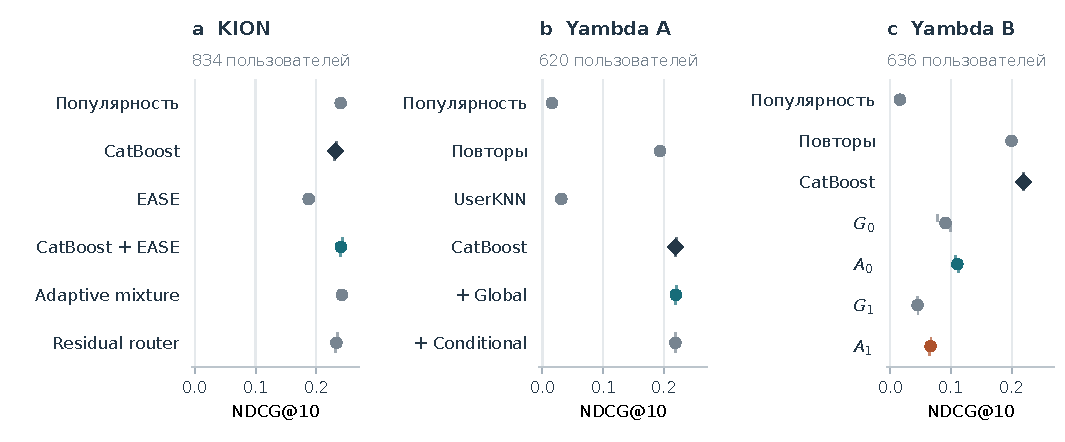
\includegraphics[width=\textwidth]{figures/model_comparison.pdf}
\caption{Абсолютное качество и сильные контроли на трёх выборках.
Крупные точки~--- user-macro средние; малые вертикальные отметки~--- метрики
трёх pipeline seed, где есть три отдельных fit. Это не доверительные интервалы.
Ромб обозначает ручной CatBoost. В KION adaptive mixture имеет лучшую тестовую
точку, но не был выбран на search. Абсолютные метрики разных панелей относятся
к разным задачам и не сравниваются напрямую.}
\label{fig:models}
\end{figure*}

\section{Результаты и интерпретация}

\begin{table*}[t]
\centering\small
\caption{Три основные гипотезы, зафиксированные до соответствующих внешних метрик.
Парные 95\% интервалы относятся к пользователям, а не к распределению новых обучений.}
\label{tab:primary}
\begin{tabular}{@{}llrrl@{}}\toprule
Выборка & Сравнение & Пользователей & $\Delta$ NDCG@10 & 95\% интервал\\\midrule
%% BEGIN GENERATED:primary-rows
KION & CatBoost + EASE -- manual & 834 & +0.00860 & $[+0.00584;+0.01188]$ \\
Yambda A & Conditional -- Global & 620 & -0.00075 & $[-0.00197;+0.00037]$ \\
Yambda B & $A_1-G_0$ & 636 & -0.02471 & $[-0.03280;-0.01652]$ \\
%% END GENERATED:primary-rows
\bottomrule\end{tabular}
\end{table*}

\subsection{Обученные признаки поверх CatBoost}
На KION гибрид EASE улучшил замороженный ручной CatBoost
с 0.23173 до 0.24033 ($\Delta=\KionDelta$).
Популярность дала 0.24000; интервал разности hybrid--popularity
$[\KionPopLow;\allowbreak\KionPopHigh]$ включает ноль.
Имеется улучшение конкретного GBDT, но не доказательство превосходства
над сильнейшим доступным контролем. Собственный residual router
также не дал убедительного выигрыша; все варианты видны на рис.~\ref{fig:models}.

На Yambda A условный фон уступил глобальному на $\ConditionalDelta$;
интервал включает ноль. Global--manual равен +0.00035
с интервалом $[-0.00073;+0.00151]$: добавочная польза не установлена.
Raw/signed графы не дают прироста. Исправление поддержки смесью noise
тоже не улучшило manual ($\MixtureDelta$;
$[\MixtureLow;\allowbreak\MixtureHigh]$).
По search выбран ручной вариант; лидер тестовой точки не становится
выбранной моделью задним числом.

\subsection{Раздельные эффекты фона и агрегации}
Основное $A_1-G_0$ на новой когорте отрицательно:
$\PrimaryDelta$ с интервалом $[\PrimaryLow;\allowbreak\PrimaryHigh]$.
Это совместное изменение двух компонентов. Их разложение
на рис.~\ref{fig:effects} показывает противоположные эффекты:
арифметическое объединение улучшает самостоятельную оценку при обоих фонах,
а добавление $\log q$ ухудшает оба правила объединения.
Взаимодействие эффектов равно +0.00200
с интервалом $[-0.00372;+0.00802]$ и не получило подтверждения.

\begin{table}[t]
\centering\small
\caption{Одинаковые векторы, история и кандидаты; меняются только
два фактора. В ячейках NDCG@10 когорты B.}
\label{tab:factorial}
\begin{tabular}{@{}lrr@{}}\toprule
Объединение & $b=0$ & $b=1$\\\midrule
%% BEGIN GENERATED:factorial-rows
Геометрическое $G$ & 0.09111 & 0.04507 \\
Арифметическое $A$ & 0.11043 & 0.06639 \\
%% END GENERATED:factorial-rows
\bottomrule\end{tabular}
\end{table}

Вторичное $A_0-G_0=\ArithmeticDelta$ не заменяет основную гипотезу.
$A_0=\AzeroShort$ остаётся значительно ниже manual
($\ManualNewShort$) и повторов ($\RepeatNewShort$).
Из 20 вариантов добавления этих оценок к ручному прогнозу на прежней валидации
лучшим оказался нулевой вес. Таким образом, улучшение одного
преобразования представления не стало улучшением полного ранжировщика.

\begin{figure*}[t]
\centering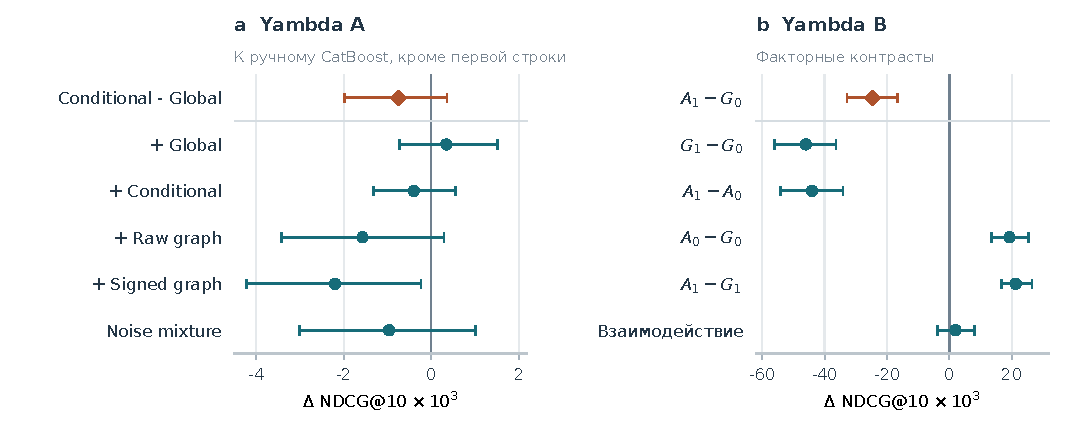
\includegraphics[width=\textwidth]{figures/paired_effects.pdf}
\caption{Парные разности NDCG@10 и 95\% user-cluster интервалы.
Оранжевым выделены заранее основные гипотезы; остальные интервалы
описательные, без поправки на множественные сравнения.
Слева первая строка сравнивает conditional и global, остальные~---
с ручным CatBoost. Справа $G/A$ и $b$ определены в~\eqref{eq:factorial};
взаимодействие равно $(A_1-A_0)-(G_1-G_0)$.
Масштабы осей различаются; единица на каждой оси соответствует $10^{-3}$ NDCG.}
\label{fig:effects}
\end{figure*}

\balance
\subsection{Диагностика границ переноса}
На старом search 93.4\% глобально шумовых пар имеют нулевую массу
условного фона; 92.6\% различных наблюдаемых рёбер встретились один раз.
Учебный AUC global/conditional равен .975/.950,
на более поздних переходах~--- .648/.562.
Последняя оценка использует 7890 положительных пар с известными обеими
ролями, 74.8\% всех поздних переходов; лишь 16.2\% этих рёбер уже встречались.
Это механистическая диагностика на когорте A, не новая подтверждающая проверка.
Разрыв смешивает временной сдвиг и смену состава рёбер;
его нельзя целиком приписать запоминанию.

Аудит после просмотра теста показал: более 54\% кандидатов A
новы для пользователя, но среднее покрытие релевантных новинок
лишь 6.5--7.1\%. Доля новинок в top-10 ручного бустинга около 0.05\%, попаданий по ним нет.
Общий NDCG здесь прежде всего характеризует повторное потребление.
Этот аудит не менял опубликованные модели и кандидаты.

\section{Ограничения и вывод}
Новые UID не заменяют новый период: A/B имеют общий сервис, дни и часть items.
Два дня и 1000 пользователей на когорту ограничивают внешний вывод.
KION хранит последнюю дату пары, а не поток повторов; накопленные длительности
и проценты просмотра исключены. Статические метаданные и задержки логирования остаются
допущениями. Отсутствующее взаимодействие не является отказом после показа;
CTR, причинный эффект и online-прирост не измеряются.

Средний вектор требует $O((L+K)d)$ операций на пользователя,
явная смесь~--- $O(LKd)$ при $L\le100$, $K\le300$, $d=64$.
Полный перебор всё ещё зависит от размера каталога; теста промышленной скорости нет.
В Yambda выполнены 120 обучений кодировщиков и 40 обучений CatBoost, включая поиск
и когорту B. Все журналы, 66 replay-прогнозов B, замены будущих событий
и пользовательские метрики доступны в репозитории. Проверка чисел не требует исходных данных или GPU.

Главный вывод: полезность contrastive-признака определяется не только
качеством proxy-loss. Фон задаёт, какую ассоциацию вычитает модель,
а объединение истории~--- как свидетельства преобразуются в ranking score.
В выполненном протоколе их раздельное изменение имеет измеримые эффекты,
но не заменяет сильные ручные признаки. Тесты открыты; дальнейший выбор
настроек требует новой внешней проверки.

\begin{thebibliography}{9}
\fontsize{8}{9.5}\selectfont\raggedright\interlinepenalty=10000\setlength{\itemsep}{1pt}\setlength{\parskip}{0pt}
\bibitem{ease} H. Steck. Embarrassingly Shallow Autoencoders for Sparse Data.
WWW, 2019. \href{https://arxiv.org/abs/1905.03375}{arXiv:1905.03375}.
\bibitem{nce} M. Gutmann, A. Hyv\"arinen. Noise-contrastive estimation: A new
estimation principle for unnormalized statistical models. AISTATS, 2010.
\href{https://proceedings.mlr.press/v9/gutmann10a.html}{PMLR 9:297--304}.
\bibitem{sgns} O. Levy, Y. Goldberg. Neural Word Embedding as Implicit Matrix
Factorization. NeurIPS, 2014.
\href{https://proceedings.neurips.cc/paper_files/paper/2014/file/b78666971ceae55a8e87efb7cbfd9ad4-Paper.pdf}{Текст статьи}.
\bibitem{poe} G. E. Hinton. Training Products of Experts by Minimizing Contrastive
Divergence. Neural Computation 14:1771--1800, 2002.
\href{https://www.cs.toronto.edu/~hinton/absps/nccd.pdf}{Текст статьи}.
\bibitem{kion} A. Petrov et al. MTS Kion Implicit Contextualised Sequential Dataset
for Movie Recommendation. 2022. \href{https://arxiv.org/abs/2209.00325}{arXiv:2209.00325}.
\bibitem{yambda} A. Ploshkin et al. Yambda-5B: A Large-Scale Multi-modal Dataset
for Ranking And Retrieval. 2025. \href{https://arxiv.org/abs/2505.22238}{arXiv:2505.22238}.
\bibitem{metrics} W. Krichene, S. Rendle. On Sampled Metrics for Item Recommendation.
KDD, 2020. \href{https://research.google/pubs/on-sampled-metrics-for-item-recommendation/}{Текст статьи}.
\end{thebibliography}
\end{document}
